% =====================================================================================================
\chapter{Data sources and physical feature extraction}\label{ch:features}
% =====================================================================================================

This chapter defines, once, every input quantity used anywhere in the project: where the raw data come from, how a raw
file becomes a number, in which unit, by which function of the code, and what happens to non-positive or missing values.
The phase chapters (\cref{ch:phase1,ch:phase2,ch:phase3,ch:phase4,ch:phase5,ch:phase6}) refer back here and only state
differences. When the description in a repository report and the code differ, the code is followed and the difference
is flagged with a \texttt{\% CHECK} comment in the \LaTeX{} source.

% -----------------------------------------------------------------------------------------------------
\section{Instruments, data modes and catalogues}\label{sec:instruments}
% -----------------------------------------------------------------------------------------------------

\Cref{tab:instruments} lists every data product that enters a model or a test. All raw files were obtained by scripts;
every download is recorded with its URL, size in bytes and SHA256 in \file{logs/downloads.jsonl} (50\,773 records,
\cref{app:reproduction}). Raw data are not in git (\file{data/raw/} is ignored, large sets live outside the repository
under \file{~/xrb-pilot-data/}).

\begin{table}[htbp]
\centering\small
\caption[Instruments, data modes and catalogues]{Instruments, data modes and catalogues used in the project. ``Versions''
gives where the product enters a model or test. Band and resolution are those actually used by the code (not the
instrument limits). Code: the function that reads or processes the product.}
\label{tab:instruments}
\begin{tabularx}{\textwidth}{@{}p{3.3cm}p{1.5cm}X p{3.1cm}@{}}
\toprule
Product & Versions & What is used & Code \\
\midrule
RXTE/PCA Standard-2 Standard Products (\texttt{xp*\_s2.pha}, \texttt{\_b2.pha}, \texttt{.rsp}) & v1--v8, v10 &
129-channel total and \texttt{pcabackest} background spectra summed over the PCUs listed in the \texttt{ROWID} keywords;
5--25\,keV (3--25\,keV in v3b); response for the same PCU combination & \file{spectra.py}: \code{read\_pha},
\code{read\_rsp}, \code{net\_spectrum}; \file{04\_fetch\_process.py} \\
RXTE/PCA Standard-1 (\texttt{pca/FS46\_*}) & v2--v10 & 0.125\,s light curves per PCU (\texttt{XeCntPcu0--4}), plus array
rates \texttt{VpCnt}, \texttt{RemainingCnt}, \texttt{VLECnt}; 128\,s rows of 1024 bins & \code{spectra.std1\_rates};
\file{v5lib.py}; \file{v6lib.py}; \file{v7lib.py} \\
RXTE/PCA event mode (\texttt{pca/SE*.evt.gz}) & v8c & Events with \texttt{TIME}, \texttt{PCUID}; modes
\texttt{E\_\{n\}us\_\{m\}M\_0\_\{k\}s}; binned at $2^{-12}$\,s & \file{v8lib.py}: \code{read\_events},
\code{hf\_features} \\
RXTE/HEXTE cluster~B Standard Products (\texttt{xh*\_s1.pha}, \texttt{\_b1.pha}) & v4b3 & Net 25--40 and 40--60\,keV
count rates & \file{19\_v4b3\_hexte.py} \\
RXTE \texttt{MissionLongData} catalogues; HEASARC TAP \texttt{xtemaster} & v1--v8 & Observation lists: \texttt{OBSID},
\texttt{TIME}, \texttt{EXPOSURE}, \texttt{STD1RATE}, \texttt{RA}, \texttt{DEC}, \texttt{NPCU} & \file{03\_select\_observations.py},
\file{20\_v4b2\_select.py}, \file{41\_v8b\_select.py} \\
MAXI/GSC standard products, 1-day light curves & v7c, v8d, v9c & Photon fluxes in 2--4, 4--10, 10--20\,keV &
\file{38\_v7c2\_select.py} \\
de Beurs et al.\ (2022) processed data (GitHub, commit \texttt{488b785}) & v7c1 & Their 44 sources, ten 20\% subsamples,
features $(\mathrm{RelInt},\mathrm{SC},\mathrm{HC})$ & \file{37\_v7c1\_repro.py} \\
NICER/XTI cleaned events (\file{ni*\_0mpu7\_cl.evt.gz}); HEASARC TAP \texttt{nicermastr} & v9--v13 & Events with
\texttt{TIME}, \texttt{PI}, \texttt{DET\_ID}; 2--10\,keV; $1/256$\,s bins, 128\,s segments & \file{v9lib.py},
\file{v10lib.py}, \file{v11lib.py} \\
NICER unfiltered events (\texttt{\_ufa}), NICER CALDB 3C50 library & v12, v13 & Input of HEASoft
\texttt{nibackgen3C50} (3C50 background model) & \file{v12\_bkg3c50.sh}, \file{58\_v12\_bkg.py}, \file{62\_v13\_bkg.py} \\
MINBAR DR1 burst, observation and source tables & v7--v9 & Burst start times and durations; burst-source positions &
\file{v7lib.py}: \code{load\_minbar}, \code{gti\_utc} \\
HI4PI (via HEASoft \texttt{nh}); XSPEC \texttt{tbabs} & v8d & Galactic $N_\mathrm{H}$ and band transmissions &
\file{v8d\_heasoft.sh}, \file{45\_v8d\_nh.py} \\
CDS Sesame (SIMBAD) positions & v4b2--v9 & Source positions for label and pointing matches & \file{20\_v4b2\_select.py},
\file{28\_v6\_select.py}, \file{38\_v7c2\_select.py} \\
\bottomrule
\end{tabularx}
\end{table}

% -----------------------------------------------------------------------------------------------------
\section{Source labels}\label{sec:labels}
% -----------------------------------------------------------------------------------------------------

The class label is a property of the \emph{source}: $y=1$ for a black hole (\BH) and $y=0$ for a neutron star (\NS).
Only labels with direct evidence are used for training and evaluation:
\begin{itemize}
\item \textbf{\BH}: a dynamical mass function (radial-velocity curve of the companion). Versions v1--v4 used the
dynamically confirmed systems of BlackCAT \citep{CorralSantana2016}; v6 added high-mass X-ray binaries from
\citet{CasaresJonker2014}; from v7 on the list of \citet{Marcel2026} (25 systems in their Table~1) is used.
\item \textbf{\NS}: type-I X-ray bursts (thermonuclear burning on a solid surface) from \citet{Galloway2008} (v1--v6) or
the MINBAR catalogue \citep{Galloway2020} (v7c onwards), or coherent accretion-powered pulsations \citep{PatrunoWatts2021}
(v6 external sources, v7c pulsar class; \citealt{Liu2006} for HMXB pulsars in v7c).
\item \textbf{BH candidates} (X-ray properties only, no dynamical mass) are never used as labels. In v3c they appear only
as prediction targets and in a label-sensitivity analysis.
\end{itemize}
The label rules of every version are summarised in \cref{tab:labelrules}; the realised source lists are given in the
phase chapters.

\begin{table}[htbp]
\centering\small
\caption[Source labelling and eligibility rules by version]{Source labelling and eligibility rules by version.
``Pointing'' is the maximum separation between an observation's pointing and the source position used.
Eligibility always also requires catalogue exposure $\ge 1000$\,s (RXTE: and \texttt{STD1RATE}~$\ge 5$\,c\,s$^{-1}$\,PCU$^{-1}$;
NICER: \texttt{nicermastr} exposure $\ge 1000$\,s).}
\label{tab:labelrules}
\begin{tabularx}{\textwidth}{@{}p{1.6cm}XXp{2.6cm}@{}}
\toprule
Version & \BH{} rule & \NS{} rule & Pointing / epoch / minimum \\
\midrule
v1 & 4 BlackCAT dynamical BHs with $\ge 30$ eligible pointings & 4 Galloway+2008 bursters & 0.1$^\circ$ from catalogue median; gain epoch 5, MJD 51677--54094 \\
v2, v3 & every BlackCAT Table~4 dynamical BH with a MissionLongData catalogue & every Galloway+2008 appendix-A source with a catalogue & 0.1$^\circ$; epoch 5 (MJD 51677--55931); $\ge 10$ eligible \\
v3c & 16 BlackCAT candidates (prediction only) & -- & as v2 \\
v4b2 & BlackCAT dynamical BHs matched by SIMBAD position & Galloway+2008 Table~3 bursters matched by position & all gain epochs; $\ge 10$ \\
v6 (external) & Casares \& Jonker (2014) HMXB BHs & Patruno \& Watts (2021) AMXPs (+ 4 slow pulsars as stress set) & 0.1$^\circ$ from SIMBAD; all epochs; $\ge 10$ \\
v7b2 & Cyg X-1, LMC X-1, LMC X-3 (Marcel+2026) & -- & 0.1$^\circ$ from SIMBAD; epoch 5; $\ge 10$ \\
v7c & Marcel+2026 Table~1 & MINBAR bursters without pulsations (NPNS); pulsars (PSR) secondary & MAXI source within 0.1$^\circ$ (Sesame; 0.3$^\circ$ fallback); $\ge 100$ daily points \\
v8b & unused Marcel+2026 BHs with RXTE data & -- & 0.1$^\circ$ from SIMBAD; all epochs; $\ge 3$ \\
v9--v13 & Marcel+2026 Table~1 (Sesame positions) & MINBAR bursters, excluding entries with another entry within 0.05$^\circ$ & target within 0.05$^\circ$; $\ge 5$ \\
\bottomrule
\end{tabularx}
\end{table}

% -----------------------------------------------------------------------------------------------------
\section{Observation eligibility and time-stratified sampling}\label{sec:sampling}
% -----------------------------------------------------------------------------------------------------

For every source the eligible pointings are sorted by time and divided into $K$ consecutive groups of (as nearly as
possible) equal size, using \code{numpy.array\_split} ($K=15$ for RXTE, $K=8$ for NICER). Inside each group the
candidates are put in a random order generated by a seeded generator; the first candidate that passes the post-download
quality rules (\cref{sec:quality}) is accepted. This keeps the sample spread over the source's history (several
outbursts, several states) and makes the choice independent of the spectrum. If a source has fewer than $K$ eligible
pointings, some groups are empty and all pointings are used. \Cref{alg:sampling} gives the procedure; the seeds are
listed in \cref{tab:seeds}.

\begin{algorithm}[htbp]
\caption{Time-stratified candidate ranking and acceptance (\file{03\_select\_observations.py} + \file{04\_fetch\_process.py};
NICER: \file{47\_v9\_select.py}, \file{55\_v11\_select.py}, \file{60\_v13\_select.py})}\label{alg:sampling}
\begin{algorithmic}[1]
\Require eligible pointings $\{(o_i, t_i)\}$ of one source, number of groups $K$, seed $\sigma$, maximum tries $M$
\State sort pointings by time $t_i$; split the index list into $K$ consecutive groups $G_1,\dots,G_K$ (\code{array\_split})
\State $\mathrm{rng} \gets \mathrm{default\_rng}(\sigma)$
\For{$b = 1,\dots,K$}
  \State $\pi \gets \mathrm{rng.permutation}(G_b)$ \Comment{rank within the group}
  \For{$r = 1,\dots,\min(M,|G_b|)$}
     \State download and process $o_{\pi_r}$; \If{all quality rules pass} accept $o_{\pi_r}$; \textbf{break} \EndIf
  \EndFor
\EndFor
\end{algorithmic}
\end{algorithm}

\begin{table}[htbp]
\centering\small
\caption[Sampling seeds and limits]{Sampling parameters. ``position'' is the 1-based position of the source in the
source list processed by the script. The global seed is \code{SEED = 42} (\file{config.py}).}
\label{tab:seeds}
\begin{tabularx}{\textwidth}{@{}p{4.2cm}Xp{4.2cm}l@{}}
\toprule
Sample & groups $K$ & seed $\sigma$ & max.\ tries $M$ \\
\midrule
RXTE v1, v2, v3c, v7b2, v8b & 15 & \code{SEED + position} & 6 \\
RXTE v4b2 new sources & 15 & \code{SEED + 100 + i} & 6 \\
RXTE v4b1 & one group per pointing (all eligible) & -- & 1 \\
NICER v9 & 8 & \code{SEED + position} & 3 \\
NICER v11 & 8 & \code{SEED + 1000 + position} & 3 \\
NICER v13 & 8 & \code{SEED + 2000 + position} & 3 \\
\bottomrule
\end{tabularx}
\end{table}

% -----------------------------------------------------------------------------------------------------
\section{RXTE/PCA Standard-2 spectra}\label{sec:pca}
% -----------------------------------------------------------------------------------------------------

\subsection{What the files contain}
The Standard Products of every ObsID contain a total (source + background) spectrum \texttt{xp<obs>\_s2.pha}, the
\texttt{pcabackest} model background spectrum \texttt{xp<obs>\_b2.pha} and the combined response \texttt{xp<obs>.rsp}.
The header inspection of \file{05\_two\_source\_check.py} (\file{reports/step2\_fits\_check.md}) established:
\texttt{HDUCLAS2/3 = TOTAL/COUNT}, column \texttt{COUNTS} in counts, \texttt{POISSERR = F} with explicit
\texttt{STAT\_ERR}, \texttt{SYS\_ERR = 0}, \texttt{BACKSCAL = AREASCAL = 1}, 129 channels, equal source and background
exposures, and the PCUs summed listed in the \texttt{ROWID$n$} keywords. The background statistical error is
$\sqrt{\text{model counts}}$; the systematic uncertainty of the background model is \emph{not} included anywhere.
Standard Products are \emph{not} deadtime corrected. \Cref{fig:step2} shows the two spectra used for this check.

\begin{figure}[htbp]
\centering
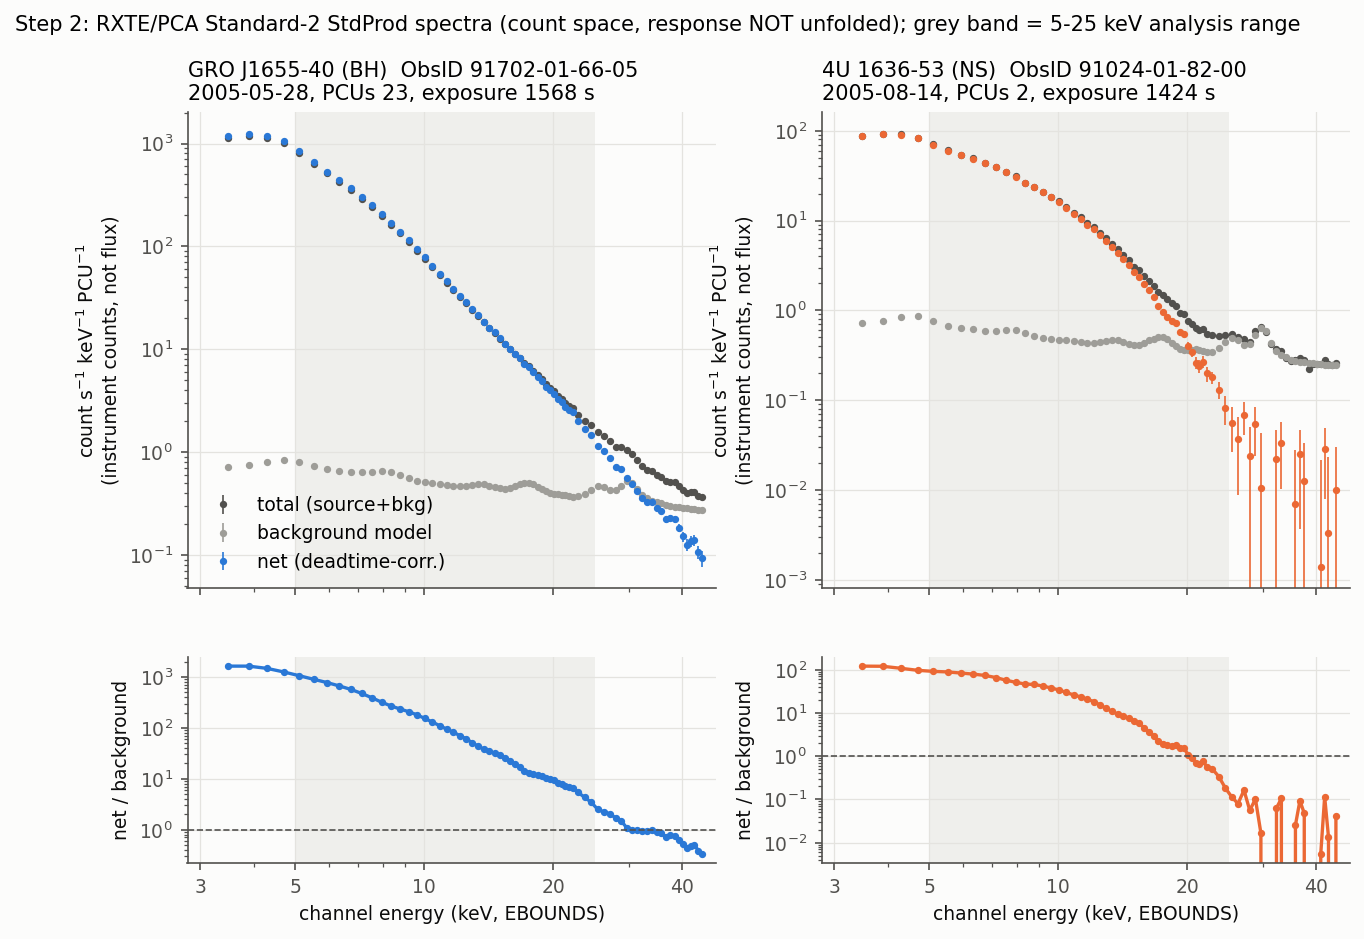
\includegraphics[width=0.92\textwidth]{figures/step2_two_sources.png}
\caption[Two Standard-2 spectra used to validate the data flow]{Data-flow validation on one \BH{} (GRO J1655$-$40,
ObsID 91702-01-66-05) and one \NS{} (4U 1636$-$53, ObsID 91024-01-82-00). Top: total (dark grey), background model
(light grey) and deadtime-corrected net (colour) count rates per keV per PCU against channel energy (EBOUNDS), log--log;
the grey band is the 5--25\,keV analysis range. Bottom: net/background ratio. The point is that the net spectrum is
background-dominated only above $\sim$30\,keV for these bright sources, and that everything is in instrument count space
(no response unfolding). Repo: \file{figures/step2\_two\_sources.png}, script \file{scripts/05\_two\_source\_check.py}.}
\label{fig:step2}
\end{figure}

\subsection{Background subtraction}\label{sec:bkg}
For channel $c$ of observation $i$, with source counts $C^{s}_{c}$ and errors $\sigma^{s}_{c}$, background counts
$C^{b}_{c}$ and errors $\sigma^{b}_{c}$ (function \code{spectra.net\_spectrum}):
\begin{align}
t_s &= \mathtt{EXPOSURE}_s\,\mathtt{AREASCAL}_s, \qquad t_b = \mathtt{EXPOSURE}_b\,\mathtt{AREASCAL}_b,\qquad
\kappa = \mathtt{BACKSCAL}_s/\mathtt{BACKSCAL}_b, \nonumber\\
r^{s}_c &= C^{s}_c/t_s,\quad e^{s}_c = \sigma^{s}_c/t_s,\qquad r^{b}_c = \kappa\,C^{b}_c/t_b,\quad e^{b}_c=\kappa\,\sigma^{b}_c/t_b, \label{eq:srcbkg}\\
r^{\mathrm{net}}_c &= D\,(r^{s}_c - r^{b}_c),\qquad e^{\mathrm{net}}_c = D\,\sqrt{(e^{s}_c)^2 + (e^{b}_c)^2}, \label{eq:net}
\end{align}
in count\,s$^{-1}$ (summed over the PCUs of the spectrum), where $D = 1/(1-\mathrm{DTF})$ is the deadtime correction factor
(\cref{sec:deadtime}). This is the OGIP/XSPEC convention: the same quantity that XSPEC uses after \texttt{data},
\texttt{backgrnd} and \texttt{response}. Non-positive net rates (possible where the source is faint, mainly at
$E>20$\,keV in soft spectra) are kept unchanged: no absolute value, no clipping, no deletion.

\subsection{Deadtime}\label{sec:deadtime}
\textbf{v1 (lower bound).} Only the good-xenon term was available from Standard-2:
\begin{equation}
\mathrm{DTF}^{(\mathrm{v1})} = 10^{-5}\,\mathrm{s}\times \frac{\sum_c C^{s}_c}{t_s\,N_\mathrm{PCU}} ,\label{eq:dtfv1}
\end{equation}
i.e.\ the total (source + background) count rate per PCU times $10\,\mu$s. Median 0.31\% and maximum 6\% in the v1
sample (\file{data/observations.csv}, column \code{dtf\_xe}).
% CHECK: report_v2_zh-TW.md states that the v1 good-xenon median was 0.15%; data/observations.csv (v1) gives 0.31% (matching
% report_zh-TW.md); 0.146% is the median of dtf_xe in the v2 sample (data/v2/observations.csv).

\textbf{v2 onwards (RXTE GOF recipe from Standard-1).} The Standard-1 files of the ObsID are read and the mean rates
inside the spectrum's good time intervals (GTIs) are computed from all 0.125\,s bins whose centre lies in a GTI
(\code{spectra.std1\_rates}): per-PCU good-xenon rates $\mathrm{Xe}_p$ ($p=0,\dots,4$) and array rates $\mathrm{Vp}$
(propane), $\mathrm{Rem}$ (coincident events) and $\mathrm{VLE}$ (very large events). With $N_\mathrm{on}$ the number of
PCUs with $\mathrm{Xe}_p > 1$\,c\,s$^{-1}$ (\code{spectra.std1\_dtf}):
\begin{equation}
\begin{split}
\mathrm{DTF}_p &= 10^{-5}\left(\mathrm{Xe}_p + \frac{\mathrm{Vp}+\mathrm{Rem}}{N_\mathrm{on}}\right) + 6\times10^{-5}\,\frac{\mathrm{VLE}}{N_\mathrm{on}},\\
\mathrm{DTF} &= \frac{1}{|\mathcal P|}\sum_{p\in\mathcal P}\mathrm{DTF}_p,\qquad D = \frac{1}{1-\mathrm{DTF}},
\end{split}\label{eq:dtf}
\end{equation}
with rates in count\,s$^{-1}$ and $\mathcal{P}$ the PCUs of the spectrum. A version with $1.5\times 10^{-4}$\,s per VLE
event (quoted elsewhere on the same GOF page) was stored only as a sensitivity number (\code{dtf\_std1\_vle150us}).
In the v2 sample the Standard-1 coverage of the spectrum GTIs has median 99\% (minimum 88\%), the DTF has median 1.38\% and
maximum 8.8\%; no observation exceeded the 10\% rule. Because $D$ multiplies the whole spectrum, it changes intensities
(representation A) by 1--9\% and leaves shapes (B, H) unchanged.

\subsection{Common energy grid and rebinning}\label{sec:grid}
Gain drifts change the channel-to-energy relation slightly between observations, so every spectrum is rebinned onto one
fixed grid defined by a reference observation (\code{REFERENCE\_OBS = 91702-01-66-05}). Let $\{E^{\mathrm{lo}}_k,
E^{\mathrm{hi}}_k\}$ be the EBOUNDS of the reference response. The grid edges are the union of all EBOUNDS edges between the
edge closest to 5\,keV and the edge closest to 25\,keV:
$e_0 = 4.908$, \dots, $e_{45} = 25.008$\,keV (45 bins, widths 0.41--0.86\,keV; \cref{tab:grid}). For v3b the lower limit
is the edge closest to 3\,keV, giving 50 bins from 2.883\,keV; the 45 bins above 4.908\,keV are identical.
For an observation with its own EBOUNDS, the overlap matrix (\code{spectra.overlap\_matrix})
\begin{equation}
W_{jk} = \frac{\max\!\bigl(0,\ \min(E^{\mathrm{hi}}_k, e_{j+1}) - \max(E^{\mathrm{lo}}_k, e_j)\bigr)}{E^{\mathrm{hi}}_k - E^{\mathrm{lo}}_k}\label{eq:overlap}
\end{equation}
is the fraction of channel $k$ that lies in grid bin $j$ (counts assumed uniform within a channel). The rebinned net
rate per keV per PCU and its error are
\begin{equation}
x_{ij} = \frac{\sum_k W_{jk}\, r^{\mathrm{net}}_{ik}}{N_{\mathrm{PCU},i}\,\Delta e_j},\qquad
\sigma_{ij} = \frac{\sqrt{\sum_k W_{jk}^2\,(e^{\mathrm{net}}_{ik})^2}}{N_{\mathrm{PCU},i}\,\Delta e_j},\qquad \Delta e_j = e_{j+1}-e_j,\label{eq:rebin}
\end{equation}
in count\,s$^{-1}$\,keV$^{-1}$\,PCU$^{-1}$ (array \code{rate} and \code{err} of \file{features.npz}). Division by the
number of PCUs is justified because the effective area grows linearly with the number of PCUs ($\approx 1070$\,cm$^2$ per
PCU at 6\,keV). The error formula treats channels as independent; two grid bins that share one channel are therefore
weakly correlated, which is ignored. The total (source + background) and background spectra are rebinned in the same
way (\code{srate}, \code{brate}). The gain drift within epoch~5 is at most 0.85 channel (median 0.17) relative to the
reference.

\begin{table}[htbp]
\centering\scriptsize
\caption[The common energy grid]{The 45-bin common energy grid (keV), from the EBOUNDS of observation 91702-01-66-05
(\file{data/v2/processed/features.npz}, key \code{edges}; identical in every RXTE sample). Bin $j$ spans $[e_j,e_{j+1})$.
The v3b grid adds five bins below: 2.883, 3.287, 3.691, 4.096, 4.502, 4.908\,keV.}
\label{tab:grid}
\setlength{\tabcolsep}{3pt}
\begin{tabular}{@{}rr@{\hspace{10pt}}rr@{\hspace{10pt}}rr@{\hspace{10pt}}rr@{\hspace{10pt}}rr@{}}
\toprule
$j$ & $e_j$ & $j$ & $e_j$ & $j$ & $e_j$ & $j$ & $e_j$ & $j$ & $e_j$\\
\midrule
0 & 4.908 & 10 & 9.001 & 20 & 13.149 & 30 & 17.346 & 40 & 21.588 \\
1 & 5.315 & 11 & 9.414 & 21 & 13.566 & 31 & 17.768 & 41 & 22.014 \\
2 & 5.722 & 12 & 9.827 & 22 & 13.985 & 32 & 18.191 & 42 & 22.441 \\
3 & 6.130 & 13 & 10.240 & 23 & 14.403 & 33 & 18.614 & 43 & 23.295 \\
4 & 6.538 & 14 & 10.654 & 24 & 14.822 & 34 & 19.038 & 44 & 24.151 \\
5 & 6.948 & 15 & 11.069 & 25 & 15.242 & 35 & 19.462 & 45 & 25.008 \\
6 & 7.357 & 16 & 11.484 & 26 & 15.662 & 36 & 19.886 & & \\
7 & 7.767 & 17 & 11.899 & 27 & 16.082 & 37 & 20.311 & & \\
8 & 8.178 & 18 & 12.315 & 28 & 16.503 & 38 & 20.736 & & \\
9 & 8.589 & 19 & 12.732 & 29 & 16.924 & 39 & 21.162 & & \\
\bottomrule
\end{tabular}
\end{table}

\subsection{Summary quantities, errors and quality rules}\label{sec:quality}
For each observation (\file{04\_fetch\_process.py}):
\begin{align}
F_i &= \sum_{j=0}^{44} x_{ij}\Delta e_j \quad[\mathrm{count\,s^{-1}\,PCU^{-1}}],\qquad
\sigma_{F,i} = \Bigl(\sum_j (\sigma_{ij}\Delta e_j)^2\Bigr)^{1/2},\qquad \mathrm{S/N}_i = F_i/\sigma_{F,i}, \label{eq:F}\\
f^{\mathrm{bkg}}_i &= \frac{\sum_j x^{b}_{ij}\Delta e_j}{\sum_j x^{s}_{ij}\Delta e_j}\quad\text{(background fraction, 5--25 keV)}.\nonumber
\end{align}
An observation is accepted only if all of the following hold (otherwise the next candidate of the same time group is
tried): all files present and readable, 129 channels, EBOUNDS cover 5--25\,keV; spectrum exposure $\ge 1000$\,s;
$\mathrm{S/N}\ge 10$; $\mathrm{DTF}\le 0.10$; header position \texttt{RA\_OBJ/DEC\_OBJ} within 0.1$^\circ$ of the
source position; all values finite. $F_i>0$ is guaranteed by the S/N rule, so the shape normalisation
(\cref{eq:B}) is always defined.

\subsection{Response check and response-normalised spectra}\label{sec:pl2}
A fixed photon spectrum $N(E)=E^{-2}$ (photon index $\Gamma=2$, no absorption, normalised to
1\,ph\,cm$^{-2}$\,s$^{-1}$\,keV$^{-1}$ at 1\,keV) is folded through each observation's response matrix $R(E,c)$ (\code{spectra.powerlaw\_folded}) and rebinned
like the data:
\begin{equation}
P_{ic} = \sum_{\ell} R_i(E_\ell,c)\int_{E^{\mathrm{lo}}_\ell}^{E^{\mathrm{hi}}_\ell} E^{-2}\,dE,\qquad
p_{ij} = \frac{\sum_c W_{jc}P_{ic}}{N_{\mathrm{PCU},i}\,\Delta e_j}\quad(\text{key \code{pl2}}).\label{eq:pl2}
\end{equation}
The across-observation scatter of $p_{ij}/\median_i p_{ij}$ measures how much the instrument response alone changes the
count spectrum: median 3.7\%, maximum 11--12.7\%, driven by the PCU combination (\cref{fig:response}). BH and NS have
similar PCU-combination mixtures (mean tilt 2.0\% vs 2.4\% in v1), so this is treated as noise rather than as a class
shortcut. From v4b2 on, $p_{ij}$ also defines the response-normalised representations R and H$_R$ (\cref{sec:reps}),
which can be compared across gain epochs.

\begin{figure}[htbp]
\centering
\begin{subfigure}{0.49\textwidth}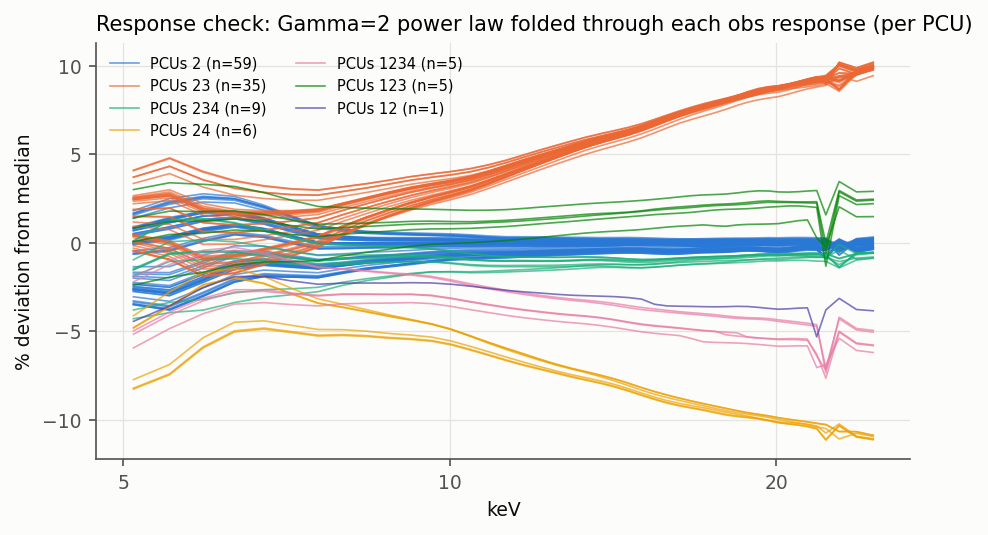
\includegraphics[width=\textwidth]{figures/step3_response_variation.png}\caption{v1 (120 observations)}\end{subfigure}
\begin{subfigure}{0.49\textwidth}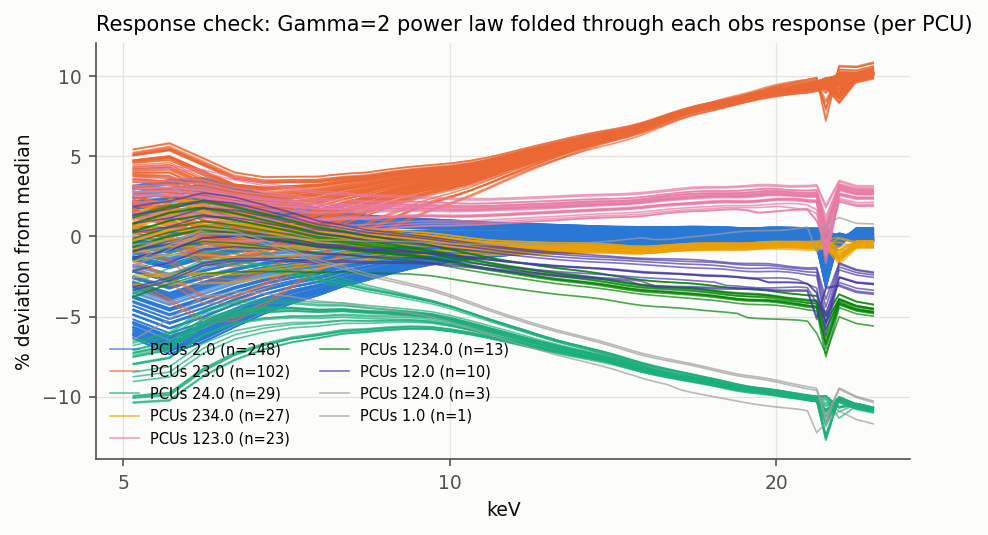
\includegraphics[width=\textwidth]{figures/v2/step3_response_variation.png}\caption{v2 (456 observations)}\end{subfigure}
\caption[Response variation between observations]{Response check: a fixed $\Gamma=2$ power law folded through each
observation's response, per PCU, shown as percentage deviation from the median over observations, against energy;
colour = PCU combination. The spread (a few per cent, up to $\sim$10\% at 25\,keV) is set by which PCUs were on, not by the
source class. Repo: \file{figures/step3\_response\_variation.png}, \file{figures/v2/step3\_response\_variation.png};
script \file{scripts/06\_dataset\_checks.py}.}
\label{fig:response}
\end{figure}

\subsection{Independent check with XSPEC}\label{sec:xspec}
For 12 randomly chosen v2 observations (seed 42; 10 sources; net rates 5--950\,c\,s$^{-1}$), HEASoft~6.37.1/XSPEC
(\texttt{data}, \texttt{backgrnd}, \texttt{response}, \texttt{ignore **-5.0 25.0-**}, \texttt{tclout rate}) and
\cref{eq:net} with $D=1$ summed over the same noticed channels (10--52 or 10--53) agree to $3\times10^{-10}$ (rate) and
$4\times10^{-10}$ (error) relative (\file{results/v2/xspec\_crosscheck.csv}, \file{scripts/10\_xspec\_crosscheck.py}). This
validates \cref{eq:srcbkg,eq:net}; it does not validate the deadtime, the rebinning, or the background model itself.

% -----------------------------------------------------------------------------------------------------
\section{Spectral representations}\label{sec:reps}
% -----------------------------------------------------------------------------------------------------

All representations are computed per observation from the rebinned spectrum $x_{i\cdot}$; none uses information from
other observations (the training-set standardisation of \cref{sec:scaler} is a separate step inside the model).
Code: \file{07\_train\_eval.py}, \code{v3lib.v2\_representations}, \file{12\_v3b\_extended\_band.py},
\code{reps\_R} in \file{22\_v4b2\_analysis.py}.

\paragraph{A (intensity kept).} With scale $a = 0.1$\,count\,s$^{-1}$\,keV$^{-1}$\,PCU$^{-1}$ (\code{ASINH\_SCALE}),
\begin{equation}
A_{ij} = \operatorname{asinh}\!\left(x_{ij}/a\right),\qquad j=0,\dots,44. \label{eq:A}
\end{equation}
$\operatorname{asinh}(u)\approx \sgn(u)\ln(2|u|)$ for $|u|\gg1$ and $\approx u$ near 0, so A is log-like for bright bins
and defined for the (rare) negative bins. A keeps the absolute count rate, which depends on distance, absorption and
accretion rate as well as on the compact object.

\paragraph{B (shape).}
\begin{equation}
B_{ij} = x_{ij}/F_i\quad[\mathrm{keV^{-1}}],\qquad \textstyle\sum_j B_{ij}\Delta e_j = 1. \label{eq:B}
\end{equation}

\paragraph{H (two count-space colours).} Four bands are formed from the grid bins whose geometric centre
$\bar e_j=\sqrt{e_je_{j+1}}$ lies in a nominal interval (\code{v3lib.band}); the exact bin ranges are in \cref{tab:bands}:
\begin{equation}
C_{i,m} = \sum_{j\in b_m} x_{ij}\Delta e_j\ \ [\mathrm{count\,s^{-1}\,PCU^{-1}}],\qquad
\vect{h}_i = (h_{i1},h_{i2}) = \left(\frac{C_{i,2}}{C_{i,1}},\ \frac{C_{i,4}}{C_{i,3}}\right). \label{eq:H}
\end{equation}
$h_1$ (``soft colour'', $\approx$\,7--10 over 5--7\,keV) and $h_2$ (``hard colour'', $\approx$\,16--25 over 10--16\,keV) are
linear ratios. The pre-registration originally specified $\log_{10}$ colours; before any v2 model was trained, two BH
spectra (95409-01-29-00 GX\,339$-$4, 60113-01-34-00 XTE J1650$-$500) were found with a slightly negative 16--25\,keV net
sum, so the linear ratio was adopted (logged in \file{reports/decision\_log.md}). Denominators $C_1, C_3$ are positive
for every observation (asserted in the code); numerators may be $\le 0$ and are kept.

\paragraph{HI, H+B, HI+A.} $\mathrm{HI}_i = (h_{i1},h_{i2},\log_{10}F_i)$; $\mathrm{H{+}B}_i = (\vect{h}_i, B_{i0},\dots,B_{i44})$
(47 features); $\mathrm{HI{+}A}_i = (\mathrm{HI}_i, A_{i0},\dots,A_{i44})$ (48 features).

\paragraph{v3b (3--25\,keV).} On the 50-bin grid: $F^{(3)}_i=\sum_{j}x_{ij}\Delta e_j$ over all 50 bins;
$\mathrm{B3}_{ij} = x_{ij}/F^{(3)}_i$; $\mathrm{H3}_i = (C_{i,0}/C_{i,1},\ C_{i,2}/C_{i,1},\ C_{i,4}/C_{i,3})$ where
$C_{i,0}$ sums the five bins with centre in $[2.8,5)$\,keV (2.883--4.908\,keV). The soft colour has 3--5\,keV in the
numerator and a denominator that is always positive.

\paragraph{R and H$_R$ (response-normalised; v4b2 onwards).} With $p_{ij}$ of \cref{eq:pl2}:
\begin{equation}
R_{ij} = \frac{x_{ij}}{p_{ij}},\qquad P_{i,m} = \sum_{j\in b_m}p_{ij}\Delta e_j,\qquad
\vect{h}^{R}_i = \left(\frac{C_{i,2}/P_{i,2}}{C_{i,1}/P_{i,1}},\ \frac{C_{i,4}/P_{i,4}}{C_{i,3}/P_{i,3}}\right). \label{eq:HR}
\end{equation}
H$_R$ is the colour of the data relative to the colour a $\Gamma=2$ power law would have through the same response; it
removes first-order response differences (e.g.\ between gain epochs). Its predictions agree with H at Spearman 0.994
(\cref{ch:phase2}).

\begin{table}[htbp]
\centering\small
\caption[Colour bands]{The four colour bands of H (and H$_R$): grid bins whose geometric centre lies in the nominal
interval, and the actual energy range they cover (computed from \code{edges}).}
\label{tab:bands}
\begin{tabular}{@{}llccc@{}}
\toprule
Band & nominal interval (centre rule) & bins $j$ & $n$ bins & actual range [keV] \\
\midrule
$b_1$ & $[5,7)$ & 0--4 & 5 & 4.908--6.948 \\
$b_2$ & $[7,10)$ & 5--11 & 7 & 6.948--9.827 \\
$b_3$ & $[10,16)$ & 12--26 & 15 & 9.827--16.082 \\
$b_4$ & $[16,25.1)$ & 27--44 & 18 & 16.082--25.008 \\
$b_0$ (v3b) & $[2.8,5)$ & 5 bins of the 50-bin grid & 5 & 2.883--4.908 \\
\bottomrule
\end{tabular}
\end{table}

\Cref{fig:meanspectra} shows the class-averaged spectra in the A, B and H representations.

\begin{figure}[htbp]
\centering
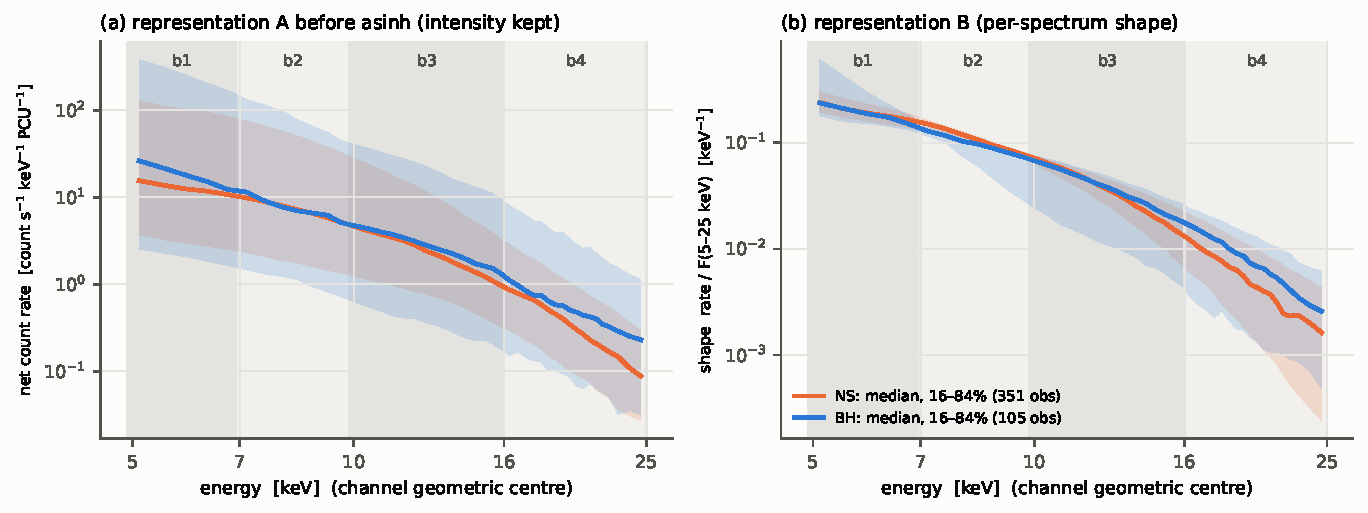
\includegraphics[width=\textwidth]{figures/generated/G2_mean_spectra.pdf}
\caption[Count-space spectra of BHs and NSs with the colour bands]{Median (line) and 16--84\% range (shading) of the
v2 count-space spectra, BH (blue, 105 observations) and NS (orange, 351 observations). (a) net rate per keV per PCU
(the quantity transformed by asinh in representation A); (b) per-spectrum shape B. Grey and light bands mark the four
colour bands $b_1$--$b_4$ of \cref{tab:bands}. Non-positive bins are omitted from the percentiles. The class medians
differ mainly in the overall slope above 10\,keV and overlap strongly, which is why two colours capture most of the
shape information (\cref{ch:phase1}). Generated for this report from \file{data/v2/processed/features.npz}
(\file{report\_en/figures/generated/make\_figures.py}).}
\label{fig:meanspectra}
\end{figure}

% -----------------------------------------------------------------------------------------------------
\section{HEXTE high-energy colours (v4b3)}\label{sec:hexte}
% -----------------------------------------------------------------------------------------------------

Only HEXTE cluster~B is used (\file{19\_v4b3\_hexte.py}), because it rocked between source and background until
2009-12-14 16:10\,UT (MJD 55179.6736); observations on or after that date, or without cluster-B files, have no HEXTE
features (60 of the 456 v2 observations). Header keyword \texttt{DEADAPP = T} (deadtime already applied) is required.
The net cluster-B spectrum follows \cref{eq:srcbkg,eq:net} with $D=1$; band rates $F_X(25\text{--}40)$ and
$F_X(40\text{--}60)$ (count\,s$^{-1}$ per cluster) use the overlap matrix of \cref{eq:overlap} on the RMF EBOUNDS. With
$F_\mathrm{PCA}(16\text{--}25)=C_{i,4}$ of \cref{eq:H}:
\begin{equation}
X_1 = \frac{F_X(25\text{--}40)}{F_\mathrm{PCA}(16\text{--}25)},\qquad X_2 = \frac{F_X(40\text{--}60)}{F_X(25\text{--}40)} .\label{eq:hexte}
\end{equation}
$X_1$ is a cross-instrument count ratio and is only used as a feature. A colour is set to missing when its denominator
has S/N $<3$ ($X_1$: 3 observations; $X_2$: 144, of which 23 BH). Missing colours are filled with the training-fold
median, and one 0/1 indicator per colour is appended (inside the LOSO loop; \code{hx\_features}); H+X therefore has 6
columns.

% -----------------------------------------------------------------------------------------------------
\section{Type-I X-ray bursts}\label{sec:bursts}
% -----------------------------------------------------------------------------------------------------

Type-I bursts are seconds-long thermonuclear flashes that only NSs produce; an observation containing one carries a
label shortcut and a distorted spectrum. Three procedures are used.

\paragraph{Standard-1 burst detector (v4; \file{17\_v4\_burst\_detect.py}).} The 1\,s light curve $r(t)$ is the sum of
good-xenon counts of the spectrum's PCUs over complete 1\,s bins inside the GTIs. With $\mu,s$ the mean and standard
deviation of all bins: candidates are bins with $r>\mu+4s$; candidates closer than 30\,s are merged into one event. For
an event with peak $r_\mathrm{pk}$ at $t_\mathrm{pk}$ and persistent level $r_0$ (median of the 60\,s before the event, or
of the whole curve if fewer than 60 bins), amplitude $A=r_\mathrm{pk}-r_0$ and levels $L_q = r_0+qA$:
\begin{equation}
\text{burst} \iff r_\mathrm{pk}\ge 1.5\,r_0\ \wedge\ t_\mathrm{rise}\le 10\,\mathrm{s}\ \wedge\ 3\le t_{1/2}\le 300\,\mathrm{s}\ \wedge\ n_{25}\ge 3,\label{eq:burst}
\end{equation}
where $t_\mathrm{rise} = t_\mathrm{pk} - \max\{t<t_\mathrm{pk}: r(t)<L_{0.25}\}$,
$t_{1/2} = \min\{t>t_\mathrm{pk}: r(t)<L_{0.5}\} - t_\mathrm{pk}$, and $n_{25}$ is the number of contiguous 1\,s bins around
the peak above $L_{0.25}$. The burst interval runs from the last time before the peak below $L_{0.25}$ to the first time
after it below $L_{0.1}$. Thresholds are \code{V4\_BURST} in \file{config.py}, following the search criterion of
\citet{Galloway2008}. Every candidate was also inspected by eye (\file{results/v4/burst\_visual.csv}).

\paragraph{MINBAR matching (v7b1; \code{v7lib.load\_minbar}, \code{gti\_utc}, \code{minbar\_flag}).} The spectrum GTIs
(\texttt{STDGTI}, mission elapsed time in TT) are converted to MJD(TT) $=\mathtt{MJDREF}+t/86400$ and then to UTC with
\texttt{astropy} (TT$-$UTC $=64.18$\,s; round-trip error $<1$\,ms). A MINBAR burst occupies $[T,\,T+\mathrm{dur}]$
(dur missing $\Rightarrow$ 300\,s). Primary rule: an observation is contaminated if a burst interval overlaps a GTI
\emph{and} the burst has the same ObsID or originates within 1$^\circ$ (PCA field of view) of the source. The literal
pre-registered rule (any burst from any origin) is kept as a sensitivity set.

\paragraph{NICER burst rule (v9--v13; \code{v9lib.burst\_events}).} The same \cref{eq:burst} is applied to the
2--10\,keV 1\,s light curve built from events inside the good intervals (\cref{sec:nicer}); every 128\,s segment that
overlaps $[t_\mathrm{start}-20\,\mathrm{s},\,t_\mathrm{end}+200\,\mathrm{s}]$ of an automatically detected burst is removed.

% -----------------------------------------------------------------------------------------------------
\section{Low-frequency timing from RXTE Standard-1 (v5--v10)}\label{sec:std1timing}
% -----------------------------------------------------------------------------------------------------

\Cref{fig:timingpipeline} summarises the chain from light curve to features; this section gives the formulae.

\begin{figure}[htbp]
\centering
\begin{tikzpicture}[every node/.style={font=\scriptsize},
  box/.style={draw=inkgrey, rounded corners=2pt, fill=boxgrey, align=center, minimum height=15mm, text width=3.45cm, inner sep=2.5pt, execute at begin node={\hyphenpenalty=10000\relax}},
  outbox/.style={box, fill=tagprim!8, draw=tagprim},
  arr/.style={-{Stealth[length=2mm]}, thick, inkgrey}]
% row 1: left to right
\node[box] (lc)    at (0,0)    {\textbf{light curves}\\ counts $c_{p,n}$, detector $p$\\ $\Delta t$ = 0.125\,s (Std-1),\\ $2^{-12}$\,s (event),\\ $1/256$\,s (NICER)};
\node[box] (seg)   at (3.95,0) {\textbf{rows / segments}\\ $N$ bins inside one GTI;\\ detector-on rule;\\ bursts removed};
\node[box] (fft)   at (7.9,0)  {\textbf{DFT per detector}\\ $X_{p,j}$, $j=0,\dots,N/2$;\\ background-corrected\\ mean counts $s_p$};
\node[box, text width=3.6cm] (cross) at (11.85,0){\textbf{all-pairs cospectrum}\\ \mbox{$C_j=\sum_{p<q}\Real\bigl(X_{p,j}X^{*}_{q,j}\bigr)$}\\ $\div\,\mathrm{sinc}^2(j/N)$\\ (closed form, \cref{eq:allpairs})};
% row 2: right to left
\node[box] (band)  at (11.85,-2.4) {\textbf{band variance}\\ per row: $\frac{2}{N^2}\sum_{j\in\mathcal B}(\cdot)$\\ $\div\sum_{p<q}s_ps_q$\\ (fractional variance $f$)};
\node[box] (agg)   at (7.9,-2.4)   {\textbf{combine rows}\\ median (Std-1, v5--v7)\\ or ratio of means\\ (event mode, NICER)};
\node[box] (feat)  at (3.95,-2.4)  {\textbf{features}\\ $T_k=\sgn(f)\sqrt{|f|}$ per band;\\ state rms; $\nu_c$ from log\\ bins; $\nu_L$ (v11c)};
\node[outbox] (dm)    at (0,-2.4)     {\textbf{design-matrix columns}\\ $T_1,T_2,T_3$ (+ missing\\ indicator); state label;\\ $\log_{10}\nu_c$ (tests)};
\draw[arr] (lc)--(seg); \draw[arr] (seg)--(fft); \draw[arr] (fft)--(cross); \draw[arr] (cross)--(band);
\draw[arr] (band)--(agg); \draw[arr] (agg)--(feat); \draw[arr] (feat)--(dm);
\end{tikzpicture}
\caption[Timing-feature pipeline]{Timing-feature pipeline shared by RXTE Standard-1 (v5--v10), RXTE event mode (v8c) and
NICER (v9--v13). Differences between the instruments are in the bin width, the segment length, the ``detector'' (PCU or
NICER MPU), whether rows are combined by the median or by the ratio of means, and the frequency bands
(\cref{tab:timingbands}). Drawn for this report.}
\label{fig:timingpipeline}
\end{figure}

\subsection{Rows, detectors and background}
A Standard-1 file stores, for each 128\,s row, $N=1024$ counts per PCU in $\Delta t = 0.125$\,s bins. Only rows lying
completely inside a spectrum GTI are used (start $\ge$ GTI start $-1$\,ms and end $\le$ GTI stop $+1$\,ms;
\code{v5lib.std1\_rows}). PCU $p$ is \emph{on} in a row if each of the eight 128-bin blocks (16\,s) has at least one count
(\code{v5lib.pcus\_on}). The background count rate per PCU is taken from the Standard-2 background spectrum over all
channels, $b = \sum_c C^b_c/(t_b N_{\mathrm{PCU},b})$ count\,s$^{-1}$ (assumed equal for all PCUs). For a detector group
or a single PCU with counts $c_n$ and $n_\mathrm{det}$ detectors, the mean \emph{source} counts per bin is
$s = \bar c - n_\mathrm{det}\, b\,\Delta t$; a row is invalid if any $s\le0$.

\subsection{Fourier conventions and the binning correction}
The discrete Fourier transform is $X_j = \sum_{n=0}^{N-1} c_n e^{-2\pi i jn/N}$, $j=0,\dots,N/2$ (\code{numpy.fft.rfft}),
frequency $\nu_j = j/(N\Delta t)$ (for 128\,s rows, $\nu_j = j/128$\,Hz). Parseval's relation gives
$\frac{1}{N}\sum_n (c_n-\bar c)^2 = \frac{1}{N^2}\sum_{j\ne0}|X_j|^2 \approx \frac{2}{N^2}\sum_{j=1}^{N/2}|X_j|^2$,
so $\frac{2}{N^2}\sum_{j\in\mathcal B}|X_j|^2$ is the variance (in counts$^2$ per bin$^2$) contributed by band
$\mathcal B$. Integrating counts over bins of width $\Delta t$ multiplies the Fourier amplitude by
$\sinc(j/N) = \sin(\pi j/N)/(\pi j/N)$ \citep[Eq.~2.19]{vanderKlis1989}; every power is divided by $\sinc^2(j/N)$.

\subsection{Two-group cospectrum (v5)}\label{sec:v5timing}
The PCUs that are on are sorted; those in even positions form group A, those in odd positions group B (at least two
PCUs are required). With $x_n,y_n$ the summed counts of the groups, $X_j,Y_j$ their transforms, and $s_x,s_y$ their
background-corrected mean source counts per bin (\code{v5lib.row\_features}):
\begin{equation}
V_\mathcal{B} = \frac{2}{N^2}\sum_{j\in\mathcal B}\frac{\Real(X_jY_j^{*})}{\sinc^2(j/N)},\qquad f_\mathcal{B} = \frac{V_\mathcal{B}}{s_x s_y} .\label{eq:v5cross}
\end{equation}
Because the Poisson (and deadtime) noise of different detectors is uncorrelated, the expected value of the cospectrum
$\Real(X_jY_j^*)$ in the absence of source variability is zero \citep{Bachetti2015,BachettiHuppenkothen2018}; no Poisson
level has to be modelled. $f_\mathcal{B}$ is the fractional variance (rms$^2$ normalised to the source mean) in band
$\mathcal B$. Per observation, the \emph{median} over valid rows is taken (robust to rare rows with flares or bursts);
fewer than 3 valid rows $\Rightarrow$ missing. Features are signed square roots,
\begin{equation}
\begin{split}
T_k &= \sgn\!\bigl(\median_r f_{k,r}\bigr)\sqrt{\bigl|\median_r f_{k,r}\bigr|},\qquad k\in\{1,2,3\},\\
T_\mathrm{tot} &= \sgn(F)\sqrt{|F|},\qquad F=\textstyle\sum_k \median_r f_{k,r},
\end{split}\label{eq:signedsqrt}
\end{equation}
(fractional rms, which may be slightly negative because of noise). The bands are listed in \cref{tab:timingbands}.
As an implementation check the conventional auto-power estimator $(|Z_j|^2 - N\bar z)/\sinc^2(j/N)$ of $z=x+y$
(Poisson level $N\bar z$, no deadtime) was also computed; for 276 S1 observations with 20--500 source c\,s$^{-1}$\,PCU$^{-1}$
the two versions of $T_2$ agree at Spearman 0.970.

\subsection{All-pairs estimator and single-PCU hybrid (v6)}\label{sec:allpairs}
Using every pair of the $n$ PCUs that are on, rather than one A/B split, reduces the noise (\code{v6lib.allpairs\_row}).
With per-PCU transforms $X_{p,j}$ and source means $s_p$:
\begin{equation}
\sum_{p<q}\Real(X_{p,j}X_{q,j}^*) = \frac{\bigl|\sum_p X_{p,j}\bigr|^2-\sum_p|X_{p,j}|^2}{2},\qquad
f_\mathcal{B} = \frac{\frac{2}{N^2}\sum_{j\in\mathcal B}\frac{|\sum_pX_{p,j}|^2-\sum_p|X_{p,j}|^2}{2\sinc^2(j/N)}}{\frac{(\sum_p s_p)^2-\sum_p s_p^2}{2}} .\label{eq:allpairs}
\end{equation}
Rows with a single PCU on use the auto-power estimator $f_\mathcal{B} = \frac{2}{N^2}\sum_{j\in\mathcal B}
\frac{|X_j|^2-N\bar c}{\sinc^2(j/N)}\big/ s^2$, but only if the total count rate is $\le 500$\,c\,s$^{-1}$ (where the
deadtime-free Poisson level is adequate); otherwise the row is invalid. $T_k^\ast$ is the signed square root of the
median over all valid rows (pair rows and single rows together). In synthetic tests the noise variance drops by 31\%,
33\% and 41\% for 3, 4 and 5 PCUs (theory 33\%, 33\%, 40\%) without bias; missing values over 8\,350 observations fall from
942 to 341.

\subsection{Characteristic frequency $\nu_c$ (v6)}\label{sec:nuc}
Nine logarithmic Fourier-index bins are formed from $\mathrm{unique}(\mathrm{round}(\mathrm{geomspace}(1,512,10)))$
$=\{1,2,4,8,\dots,512\}$ as $[1,1],[2,3],[4,7],\dots,[256,511]$ (\cref{tab:nucbins}). For each bin $b$, $P_b$ is the
median over rows of the fractional variance (\cref{eq:allpairs}) in that bin; the bin centre is
$\nu_b=\sqrt{j_\mathrm{lo}j_\mathrm{hi}}/128$\,Hz and its width in $\ln\nu$ is
$\Delta_b = \ln\bigl((j_\mathrm{hi}+0.5)/(j_\mathrm{lo}-0.5)\bigr)$. The $\nu P_\nu$ centroid is (\code{v6lib.nu\_centroid})
\begin{equation}
\ln\nu_c = \frac{\sum_b w_b\ln\nu_b}{\sum_b w_b},\qquad w_b = \frac{\max(P_b,0)}{\Delta_b},\label{eq:nuc}
\end{equation}
missing if $T^\ast_\mathrm{tot}<0.05$ or $\sum_b w_b\le0$. Since $P_b/\Delta_b$ is the power per unit $\ln\nu$ (i.e.\
$\nu P_\nu$), $\nu_c$ is the frequency around which most of the variability power per logarithmic frequency interval lies:
a model-free proxy for a break or characteristic frequency. Synthetic sinusoids at 0.05, 0.5 and 3\,Hz are recovered
within one log bin.

\begin{table}[htbp]
\centering\small
\caption[Timing frequency bands]{Fourier-index bands and their frequencies. Standard-1 and NICER use 128\,s rows or
segments ($\nu_j=j/128$\,Hz); RXTE event mode uses 16\,s segments ($\nu_j=j/16$\,Hz). From \file{config.py}.}
\label{tab:timingbands}
\begin{tabular}{@{}lllll@{}}
\toprule
Band & index $j$ & frequency [Hz] & data & config name \\
\midrule
$T_1$ & 2--12 & 0.0156--0.094 & Std-1, NICER & \code{V5\_BANDS\_J}, \code{V9\_T\_BANDS\_J} \\
$T_2$ & 13--128 & 0.102--1.000 & Std-1, NICER & \\
$T_3$ & 129--511 & 1.008--3.992 & Std-1, NICER & \\
state (v7a) & 13--511 & 0.102--3.992 & Std-1 & \code{V7\_RMS\_J} \\
state (v9+) & 13--1280 & 0.102--10.0 & NICER & \code{V9\_STATE\_J} \\
white monitor & 12288--16383 & 96--128 & NICER & \code{V9\_WHITE\_J} \\
LC & 16--63 & 1.0--3.94 & event mode & \code{V8\_HF\_BANDS\_J} \\
HF1 & 64--1023 & 4.0--63.9 & event mode & \\
HF2 & 1024--8191 & 64--512 & event mode & \\
HF3 & 8192--16383 & 512--1024 & event mode & \\
NULL & 24576--32767 & 1536--2048 & event mode & \\
\bottomrule
\end{tabular}
\end{table}

\begin{table}[htbp]
\centering\small
\caption[Bins of the $\nu P_\nu$ centroid]{Bins of the $\nu P_\nu$ centroid. Left: RXTE Standard-1 (v6; 9 bins, $\nu_b$ and
$\Delta_b$ of \cref{eq:nuc}). Right: NICER (v9--v13; 13 octave bins $j\in[2^k,2^{k+1}-1]$, centre $2^{k+0.5}/128$\,Hz).
Computed from the code (\file{v6lib.py}, \file{v9lib.py}).}
\label{tab:nucbins}
\begin{tabular}{@{}rrrr@{\hspace{18pt}}rrr@{}}
\toprule
\multicolumn{4}{c}{Standard-1 (v6)} & \multicolumn{3}{c}{NICER (v9+)}\\
\cmidrule(r){1-4}\cmidrule(l){5-7}
$[j_\mathrm{lo},j_\mathrm{hi}]$ & $\nu_b$ [Hz] & range [Hz] & $\Delta_b$ & $k$ & $[j_\mathrm{lo},j_\mathrm{hi}]$ & $\nu_k$ [Hz]\\
\midrule
$[1,1]$ & 0.0078 & 0.0039--0.0117 & 1.099 & 0 & $[1,1]$ & 0.011 \\
$[2,3]$ & 0.0191 & 0.0117--0.0273 & 0.847 & 1 & $[2,3]$ & 0.022 \\
$[4,7]$ & 0.0413 & 0.0273--0.0586 & 0.762 & 2 & $[4,7]$ & 0.044 \\
$[8,15]$ & 0.0856 & 0.0586--0.121 & 0.726 & 3 & $[8,15]$ & 0.088 \\
$[16,31]$ & 0.174 & 0.121--0.246 & 0.709 & 4 & $[16,31]$ & 0.177 \\
$[32,63]$ & 0.351 & 0.246--0.496 & 0.701 & 5 & $[32,63]$ & 0.354 \\
$[64,127]$ & 0.704 & 0.496--0.996 & 0.697 & 6 & $[64,127]$ & 0.707 \\
$[128,255]$ & 1.411 & 0.996--1.996 & 0.695 & 7 & $[128,255]$ & 1.414 \\
$[256,511]$ & 2.826 & 1.996--3.996 & 0.694 & 8 & $[256,511]$ & 2.828 \\
 & & & & 9--12 & $[512,1023]$--$[4096,8191]$ & 5.66, 11.3, 22.6, 45.3 \\
\bottomrule
\end{tabular}
\end{table}

\subsection{State index (v7a)}\label{sec:state}
The variability state of an observation is classified by its fractional rms in 0.1--4\,Hz ($j=13$--511), computed with
\cref{eq:allpairs} from rows with $\ge2$ PCUs only (no single-PCU rows, because their Poisson level would need a deadtime
model), after removing every row that overlaps a burst interval $[t_\mathrm{start}-20\,\mathrm{s},\ \text{end}]$ (MINBAR
field-of-view rule and the v4 detector; \code{v7lib.state\_rms}). With $\rho = \sgn(\median_r f)\sqrt{|\median_r f|}$:
\begin{equation}
\text{state} = \begin{cases}\text{hard-like} & \rho>0.10\\ \text{soft-like} & \rho<0.075\\ \text{intermediate} & \text{otherwise}\end{cases}
\qquad(\text{unknown if fewer than 3 rows}),\label{eq:state}
\end{equation}
the thresholds of \citet[Table 2]{RemillardMcClintock2006}, which are defined for 0.1--10\,Hz; the 4\,Hz Nyquist limit
of Standard-1 makes $\rho$ slightly low and the hard-like class conservative. NICER (v9 onwards) uses the full
0.1--10\,Hz band. ``Soft-like/hard-like'' are operational variability classes, not full spectral-state assignments.

% -----------------------------------------------------------------------------------------------------
\section{High-frequency timing from RXTE event mode (v8c)}\label{sec:eventmode}
% -----------------------------------------------------------------------------------------------------

An event file qualifies if \texttt{DATAMODE} matches \texttt{\^{}E\_\textbackslash d+us\_\textbackslash d+M\_0\_\textbackslash d+s\$},
\texttt{TDDES2} contains the six anode chains \texttt{X1L\^{}X1R\^{}X2L\^{}X2R\^{}X3L\^{}X3R}, \texttt{TIMEDEL}~$\le2^{-12}$\,s and a
\texttt{PCUID} column exists (\code{v8lib.mode\_qualifies}); if several modes qualify, the one with the largest total size
is used. Events are binned at $\Delta t=2^{-12}$\,s (Nyquist 2048\,Hz) in 16\,s segments ($N=65536$) lying completely in
(spectrum GTI) $\cap$ (event-file GTI) and not overlapping a burst interval. A PCU is on if each of the 16 one-second
sub-intervals has an event; $\ge2$ PCUs are required. For segment $r$, with \cref{eq:allpairs},
$\mathrm{num}_{\mathcal B,r} = \frac{2}{N^2}\sum_{j\in\mathcal B}\mathrm{cross}_j$ and
$\mathrm{den}_r=\sum_{p<q}s_ps_q$. The pre-registered per-observation estimator was the mean of the per-segment ratios;
because single 16\,s segments of faint sources give unstable ratios (one Aql X-1 segment gave $-195$), it was replaced,
after the implementation check IC4 and before any model, by the ratio of means with a delta-method standard error
(\code{v8lib.hf\_summary}):
\begin{equation}
\hat R_\mathcal{B} = \frac{\sum_r \mathrm{num}_{\mathcal B,r}}{\sum_r \mathrm{den}_r},\qquad
\widehat{\mathrm{SE}}(\hat R_\mathcal{B}) = \frac{1}{\sum_r\mathrm{den}_r}\sqrt{\frac{n}{n-1}\sum_r\bigl(\mathrm{num}_{\mathcal B,r}-\hat R_\mathcal{B}\,\mathrm{den}_r\bigr)^2},\label{eq:ratioofmeans}
\end{equation}
with $n$ segments; features are $\sgn(\hat R)\sqrt{|\hat R|}$ for LC, HF1, HF2, HF3. Quality: $n\ge10$ and
$|z_\mathrm{NULL}|=|\hat R_\mathrm{NULL}/\widehat{\mathrm{SE}}|\le5$ in the empty 1536--2048\,Hz band. A post hoc
correction subtracts the null-band power scaled by bandwidth from every band
($\hat R_\mathcal{B}-\hat R_\mathrm{NULL}\,|\mathcal B|/|\mathrm{NULL}|$), because a white cross-PCU correlated component
was found (\cref{ch:phase4}).

% -----------------------------------------------------------------------------------------------------
\section{NICER/XTI features (v9--v13)}\label{sec:nicer}
% -----------------------------------------------------------------------------------------------------

\subsection{Reading the events}
Cleaned event files are read without HEASoft by a streaming FITS parser (\code{v9lib.PrefixParser}) that decompresses
the gzip stream and extracts \texttt{TIME}, \texttt{PI} and \texttt{DET\_ID} from the binary table rows. Three reading
modes were used: v9 downloaded only the \emph{prefix} of each file (HTTP range requests) until $\ge6$ gap-free 128\,s
segments, end of file, or 300\,MB; v10 appended the \emph{tail} up to 1\,GB compressed and parsed prefix + tail as one
stream; v11 and v13 \emph{streamed} whole files (up to 1\,GB) into memory without storing them. Parsing was checked to be
identical to \texttt{astropy} and across the three modes (IC1 of v9--v11).

\subsection{Good intervals, segments and detectors}
Good intervals are maximal stretches without a gap $>1$\,s between consecutive events of any energy
(\code{v9lib.good\_intervals}). Each good interval $[a,b]$ is cut sequentially into 128\,s segments starting at $a$.
Only 2--10\,keV events are used for timing (PI 200--999, PI in units of 10\,eV). The detector unit is the MPU,
$m=\lfloor\mathtt{DET\_ID}/10\rfloor\in\{0,\dots,6\}$. Events are binned at $\Delta t = 1/256$\,s ($N=32768$, Nyquist
128\,Hz). MPU $m$ is on in a segment if each of the eight 16\,s blocks has a 2--10\,keV event; $\ge2$ MPUs are required.
Segments overlapping a burst interval (\cref{sec:bursts}) are removed.

\subsection{Per-segment statistics and observation features}
For each valid segment $r$ (\code{v9lib.segment\_stats}): $s_m$ is the mean 2--10\,keV counts per bin of MPU $m$ (no
background subtraction), the all-pairs cross-power is formed as in \cref{eq:allpairs}, and for each band
$\mathrm{num}_{\mathcal B,r}=\frac{2}{N^2}\sum_{j\in\mathcal B}\mathrm{cross}_j$, $\mathrm{den}_r=\sum_{m<m'}s_ms_{m'}$.
Observation features use the ratio of means (\cref{eq:ratioofmeans}) for $T_1,T_2,T_3$, the state band 0.1--10\,Hz and the
96--128\,Hz white monitor, and the signed square root. In addition:
\begin{itemize}
\item \textbf{Colours} (\code{c1}, \code{c2}): counts of \emph{all} events in the accepted segment windows in PI 200--399
($A$, 2--4\,keV), 400--599 ($B$, 4--6\,keV) and 600--999 ($C$, 6--10\,keV); $c_1=B/A$, $c_2=C/B$.
\item \textbf{Count rate} \code{rate\_2\_10}: mean over segments of the 2--10\,keV counts of the MPUs that are on, divided
by 128\,s.
\item \textbf{$\nu_c$}: 13 octave bins $k=0,\dots,12$ with $j\in[2^k,2^{k+1}-1]$ (1/128--64\,Hz, \cref{tab:nucbins});
$\ell_k=\sum_r\mathrm{num}_{k,r}/\sum_r\mathrm{den}_r$; $\nu_c=\exp\bigl(\sum_k w_k\ln\nu_k/\sum_kw_k\bigr)$ with
$w_k=\max(\ell_k,0)$ and $\nu_k = 2^{k+0.5}/128$\,Hz; missing if $\sqrt{\max(\sum_k\ell_k,0)}<0.05$.
% CHECK: preregistration_v9.md says nu_c uses "the v6 definition"; v9lib.obs_features weights the octave bins by max(l_k,0)
% without dividing by the bin width in ln(nu) (v6 divides by Delta_b). For octave bins Delta_b is ~ln 2 for every bin except
% k = 0 (ln 3), so the two definitions differ only through the lowest bin.
\item \textbf{State}: \cref{eq:state} applied to the 0.1--10\,Hz rms.
\item \textbf{Quality}: at least 3 valid segments and \code{rate\_2\_10}~$\ge20$\,c\,s$^{-1}$ (background then
$\lesssim5\%$ by the pre-registered estimate).
\end{itemize}

\subsection{Background proxy (v10)}
$\beta_i = N(\mathrm{PI}\ 1200\text{--}1499)/N(\mathrm{PI}\ 200\text{--}999)$, the 12--15\,keV to 2--10\,keV event ratio of the
whole file (\code{v10lib.bkg\_ratio}); the source contributes little above 12\,keV, so a high $\beta$ indicates
background. The threshold is the 99th percentile of $\beta$ among observations with \code{rate\_2\_10}~$\ge500$\,c\,s$^{-1}$
(where background is negligible); it was frozen at 0.2687 and reused in v11.

\subsection{3C50 background correction and screening (v12, v13)}\label{sec:3c50}
For observations with \code{rate\_2\_10}~$<500$\,c\,s$^{-1}$, HEASoft \texttt{nibackgen3C50} \citep{Remillard2022} was run
inside WSL with default parameters and the NICER CALDB (\file{scripts/v12\_bkg3c50.sh}); it returns a total spectrum
$T(\mathrm{PI})$ and a background spectrum $B(\mathrm{PI})$. Band background fractions are
$f_\mathcal{X}=\sum_{\mathcal X}B/\sum_{\mathcal X}T$ for $\mathcal X\in\{A,B,C,\text{T}=200\text{--}999\}$. Brighter
observations get $f=0$. The frozen correction (\code{corrected} in \file{59\_v12\_analysis.py}, copied verbatim into
\file{63\_v13\_analysis.py}) is
\begin{equation}
T_k' = \frac{T_k}{1-f_\mathrm{T}}\ (k=1,2,3,\text{state}),\qquad
c_1' = \frac{B(1-f_B)}{A(1-f_A)},\qquad c_2' = \frac{C(1-f_C)}{B(1-f_B)},\label{eq:3c50}
\end{equation}
followed by re-classification of the state; $\nu_c$ is not changed (it depends only on the shape of the power spectrum).
The first relation holds because a fractional rms is normalised to the total mean; normalising to the source mean
$S=(1-f)(S+B)$ multiplies it by $1/(1-f)$ (assuming a constant background). Screening keeps an observation if it is bright,
or if 3C50 succeeded and $f_\mathrm{T}\le0.20$. 3C50 failures (mostly data processed with the oldest gain calibration,
which the tool rejects) are excluded. In v13 a descriptive variant recomputed the faint observations' features from
events inside the GTIs of the 3C50 total spectrum only (\code{gti\_restricted} in \file{63\_v13\_analysis.py}).

\subsection{Lorentzian fits (v11c)}\label{sec:lorentz}
The 13 octave-bin fractional variances $\ell_k$ (with delta-method errors, \code{v11lib.lb\_se}) are fitted by one or two
zero-centred Lorentzians whose integrated variance in a bin $[\nu^{\mathrm{lo}}_k,\nu^{\mathrm{hi}}_k]$ (bin edges
$(j\mp0.5)/128$\,Hz) is
\begin{equation}
L_k(r^2,\Delta) = r^2\,\frac{2}{\pi}\left[\arctan\frac{\nu^{\mathrm{hi}}_k}{\Delta}-\arctan\frac{\nu^{\mathrm{lo}}_k}{\Delta}\right],
\qquad \Delta\in[1/128,\,128]\ \mathrm{Hz}, \label{eq:lorentz}
\end{equation}
by weighted least squares in log-parameters (\code{scipy.optimize.least\_squares}, four starting points each,
\code{v11lib.fit\_lorentz}); $\mathrm{BIC}=\chi^2+k\ln n$ with $k=2$ or 4 parameters; two components are preferred if
$\mathrm{BIC}_1-\mathrm{BIC}_2>6$. The width of the lowest-frequency component, $\nu_L$, is the ``break'' frequency.

% -----------------------------------------------------------------------------------------------------
\section{MAXI/GSC features (v7c, v8d, v9c)}\label{sec:maxi}
% -----------------------------------------------------------------------------------------------------

The MAXI 1-day standard light curve of a source gives photon fluxes $L$ (2--4\,keV), $M$ (4--10\,keV), $H$
(10--20\,keV) and errors. Points are kept if every band has $\mathrm{flux}/\mathrm{error}\ge\sqrt3$ and positive
errors, then points with $L+M+H \ge \overline{(L+M+H)}+10\,\mathrm{sd}$ are dropped; sources need $\ge100$ points
\citep[cuts of][]{deBeurs2022}. Features per point (\file{39\_v7c2\_analysis.py}):
\begin{equation}
\mathrm{SC}=\frac{M-L}{M+L},\quad \mathrm{HC}=\frac{H-L}{H+L},\quad C_4=\frac{H-M}{H+M},\quad
\mathrm{RelInt}=\frac{L+M+H}{Q_{99.99}(L+M+H)} ,\label{eq:maxi}
\end{equation}
where $Q_{99.99}$ is the 99.99th percentile over that source's points. Feature sets: CCI = (SC, HC, RelInt), C2D = (SC, HC)
and C1D = ($C_4$), the only colour without 2--4\,keV.

\paragraph{$N_\mathrm{H}$ correction (v8d; \file{45\_v8d\_nh.py}, \file{v8d\_heasoft.sh}).} The Galactic HI column
$N_\mathrm{H}$ at each source position is the HI4PI \citep{HI4PI2016} weighted average within 0.1$^\circ$ (HEASoft
\texttt{nh}, output \texttt{avwnh}). XSPEC computes photon fluxes of \texttt{tbabs*powerlaw} ($\Gamma=2$; \texttt{abund
wilm}, \texttt{xsect vern}; \citealt{Wilms2000}) on a grid $N_\mathrm{H}\in\{0\}\cup\{10^{19},\dots,10^{23.5}\}$\,cm$^{-2}$
(200 log steps); the transmission is $t_\mathcal{X}(N_\mathrm{H}) = \Phi_\mathcal{X}(N_\mathrm{H})/\Phi_\mathcal{X}(0)$
(e.g.\ 0.864, 0.979, 0.997 in $L,M,H$ at $10^{22}$\,cm$^{-2}$), interpolated linearly in $\log N_\mathrm{H}$. Corrected
fluxes $L'=L/t_L$, $M'=M/t_M$, $H'=H/t_H$ give $\mathrm{SC}'$, $\mathrm{HC}'$, $C_4'$, $\mathrm{RelInt}'$ by
\cref{eq:maxi} (sets C2D\_NH, C1D\_NH, CCI\_NH).

% -----------------------------------------------------------------------------------------------------
\section{Feature summary}\label{sec:featsummary}
% -----------------------------------------------------------------------------------------------------

\Cref{tab:featsummary} summarises all features, their units, defining equations and producing scripts.

\begin{longtable}{@{}p{2.3cm}p{1.6cm}p{2.8cm}p{4.3cm}p{3.3cm}@{}}
\caption[Summary of all features]{Summary of every feature that enters a model or test. Missing-value rule:
``excluded'' = the observation does not enter; ``median+ind.'' = training-fold median and 0/1 indicator
(\cref{sec:missing}); ``term = 0'' = CCTLR timing term set to zero.}\label{tab:featsummary}\\
\toprule
Feature & Unit & Definition & Code & Non-positive / missing \\
\midrule\endfirsthead
\toprule Feature & Unit & Definition & Code & Non-positive / missing \\ \midrule\endhead
\bottomrule\endfoot
$x_{ij}$ (\code{rate}) & c/s/keV/\allowbreak PCU & \cref{eq:rebin} & \file{04\_fetch\_process.py} & kept as is \\
$A_{ij}$ & -- & \cref{eq:A} & \code{v2\_representations} & asinh defined for $<0$ \\
$B_{ij}$ & keV$^{-1}$ & \cref{eq:B} & same & $F>0$ guaranteed \\
$h_1,h_2$ & -- & \cref{eq:H} & same & denominators $>0$; numerators kept \\
$\log_{10}F$ & dex & \cref{eq:F} & same & $F>0$ \\
B3, H3 & -- & \cref{sec:reps} & \file{12\_v3b\_extended\_band.py} & as above \\
$R_{ij}$, $h^R_{1,2}$ & -- & \cref{eq:HR} & \code{reps\_R} & as above \\
$X_1,X_2$ & -- & \cref{eq:hexte} & \file{19\_v4b3\_hexte.py} & S/N$<3$ $\to$ median+ind. (per colour) \\
$T_1,T_2,T_3$ (v5) & frac.\ rms & \cref{eq:v5cross,eq:signedsqrt} & \code{v5lib.obs\_timing} & $<3$ rows $\to$ median+ind. \\
$T^\ast_k$ (v6) & frac.\ rms & \cref{eq:allpairs} & \code{v6lib.obs\_timing\_v6} & median+ind.; CCTLR: term = 0 \\
$\nu_c$ (RXTE) & Hz & \cref{eq:nuc} & \code{v6lib.nu\_centroid} & missing $\to$ observation not in test \\
state rms (v7a) & frac.\ rms & \cref{eq:state} & \code{v7lib.state\_rms} & $<3$ rows $\to$ ``unknown'' \\
LC, HF1--3 & frac.\ rms & \cref{eq:ratioofmeans} & \code{v8lib.hf\_features} & QC fail $\to$ excluded \\
$c_1,c_2$ (NICER) & -- & \cref{sec:nicer} & \code{v9lib.obs\_features} & excluded if QC fails \\
$T_k$, state (NICER) & frac.\ rms & \cref{eq:ratioofmeans} & same & excluded if QC fails \\
$\nu_c$ (NICER) & Hz & \cref{sec:nicer} & same & missing $\to$ not in test \\
$\beta$ & -- & \cref{sec:nicer} & \code{v10lib.bkg\_ratio} & -- \\
$f_A,f_B,f_C,f_\mathrm{T}$ & -- & \cref{eq:3c50} & \file{58\_v12\_bkg.py} & 3C50 failure $\to$ excluded \\
$\nu_L$ & Hz & \cref{eq:lorentz} & \code{v11lib.fit\_lorentz} & fit failure $\to$ missing \\
SC, HC, $C_4$, RelInt & -- & \cref{eq:maxi} & \file{39\_v7c2\_analysis.py} & cuts in \cref{sec:maxi} \\
SC$'$, HC$'$, $C_4'$ & -- & \cref{sec:maxi} & \file{45\_v8d\_nh.py} & -- \\
\end{longtable}
